\documentclass[a4paper,12pt]{memoir}
\usepackage{graphicx}
\usepackage{libertine}
\setlxvchars[\normalfont\normalsize]
\settypeblocksize{*}{\lxvchars}{1.61803398875}
\checkandfixthelayout
\begin{document}
\begin{figure}%
  \noindent
  \begin{minipage}{0.5\textwidth}%
    %\showthe\linewidth  % 165.5pt
    % But note that Ipe uses 72 points per inch
    % whereas TeX uses 72.27 points per inch,
    % so the Ipe figure must be at most 165.5 * (72 / 72.27) points wide.
    \rule{0pt}{1pt}\par
    \noindent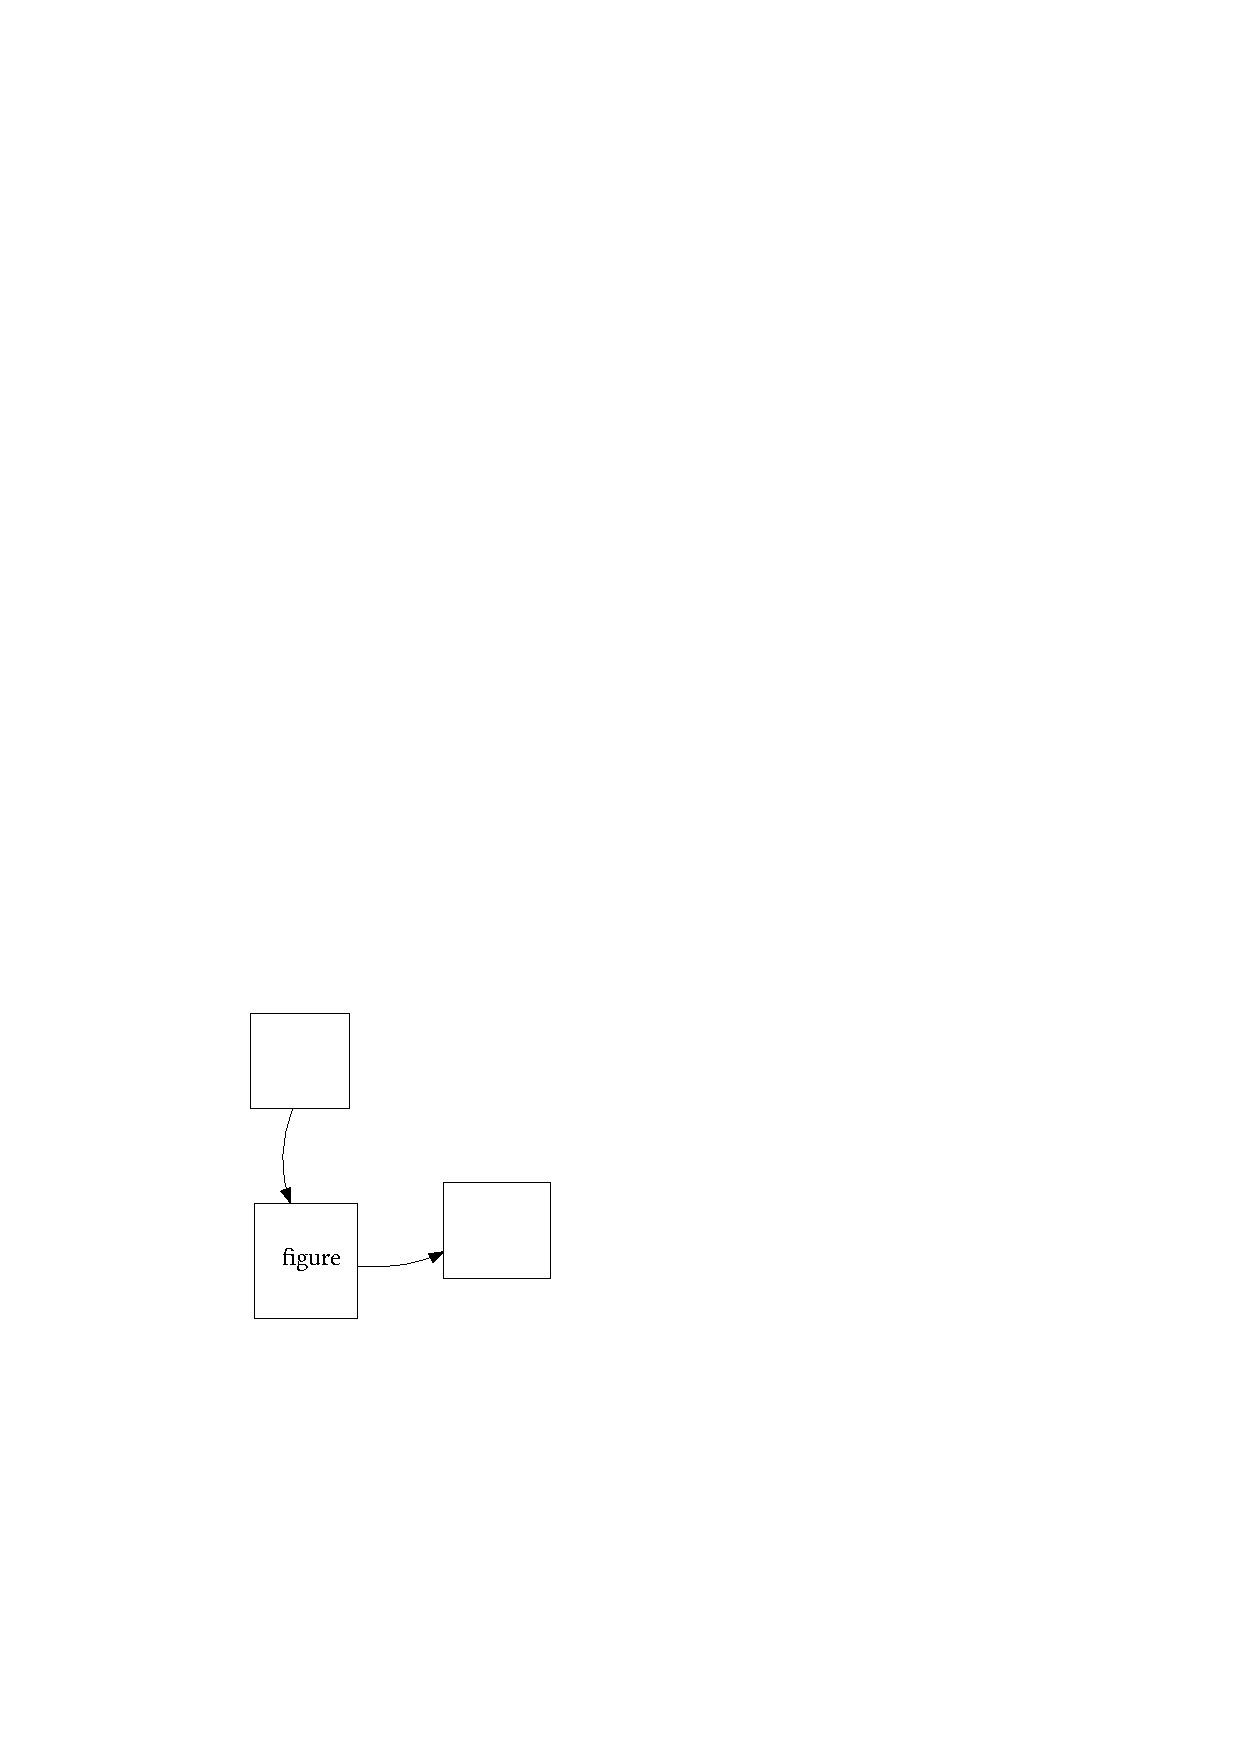
\includegraphics[scale=1,page=1]{myfigure.pdf}\par
    \rule{\linewidth}{1pt}\par
  \end{minipage}%
  \begin{minipage}{0.5\textwidth}%
    \rule{\linewidth}{1pt}\par
    \noindent\includegraphics[scale=1,page=2]{myfigure.pdf}\par
    \rule{0pt}{1pt}\par
  \end{minipage}%
  \par
  \caption{Amazing figure! wow!}
\end{figure}
\end{document}
